% REMEMBER TO SET LANGUAGE!
\documentclass[a4paper,10pt,english]{article}
\usepackage[utf8]{inputenc}
\usepackage[norsk]{babel}
% Standard stuff
\usepackage{amsmath,graphicx,varioref,verbatim,amsfonts,geometry,libertine,siunitx,float}
% colors in text
\usepackage[usenames,dvipsnames,svgnames,table]{xcolor}
% Hyper refs
\usepackage[colorlinks]{hyperref}

% Document formatting
\setlength{\parindent}{0mm}
\setlength{\parskip}{1.5mm}

%Color scheme for listings
\usepackage{textcomp}
\definecolor{listinggray}{gray}{0.9}
\definecolor{lbcolor}{rgb}{0.9,0.9,0.9}

%Listings configuration
\usepackage{listings}
%Hvis du bruker noe annet enn python, endre det her for å få riktig highlighting.
\lstset{
	backgroundcolor=\color{lbcolor},
	tabsize=4,
	rulecolor=,
	language=python,
        basicstyle=\scriptsize,
        upquote=true,
        aboveskip={1.5\baselineskip},
        columns=fixed,
	numbers=left,
        showstringspaces=false,
        extendedchars=true,
        breaklines=true,
        prebreak = \raisebox{0ex}[0ex][0ex]{\ensuremath{\hookleftarrow}},
        frame=single,
        showtabs=false,
        showspaces=false,
        showstringspaces=false,
        identifierstyle=\ttfamily,
        keywordstyle=\color[rgb]{0,0,1},
        commentstyle=\color[rgb]{0.133,0.545,0.133},
        stringstyle=\color[rgb]{0.627,0.126,0.941}
        }
        
\newcounter{subproject}
\renewcommand{\thesubproject}{\alph{subproject}}
\newenvironment{subproj}{
\begin{description}
\item[\refstepcounter{subproject}(\thesubproject)]
}{\end{description}}

%Lettering instead of numbering in different layers
%\renewcommand{\labelenumi}{\alph{enumi}}
%\renewcommand{\thesubsection}{\alph{subsection}}

%opening
\title{FYS-MEK1110 - Oblig 1}
\author{Tommy Ryan}
\date{Last modified \today}

\begin{document}

\maketitle

\section{Modeling a 100 m race}

In this project we will develop an advanced model for the motion of a sprinter during a 100 m race. We will build the model gradually, adding complications one at a time to develop a realistic model for the race

\subsection*{a) Free-body diagram}

\begin{figure}[h!]
        \centering 
        %Scale angir størrelsen på bildet. Bildefilen må ligge i samme mappe som tex-filen. 
        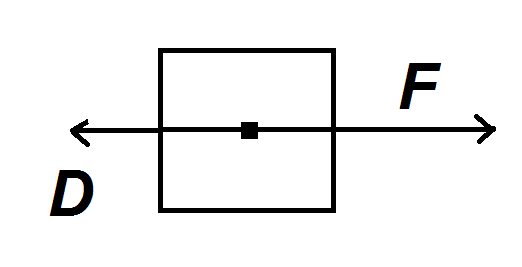
\includegraphics[scale=0.8]{a.png} 
        \caption{Free-body diagram of the sprinter.}
        %Label gjør det enkelt å referere til ulike bilder.
        \label{fig:a}
\end{figure}

%Referanser fungerer først når du har kompilert to ganger!
In figure \ref{fig:a} we see the free-body diagram of the sprinter. $F$ is the force generated by the sprinter that makes him accelerate and move forward. $D$ is the wind resistance. As can be seen in the figure, the driving force is greater in magnitude than the air resistance. This means that the sprinter will be able to move forward. 


\subsection*{b) Position $x(t)$ as a function of time}

The acceleration is constant, so we can use the equations of motion.
We know that the velocity of an object is 
\[v(t)=at.\]
To find the position, $x(t)$, we need to integrate:
\[x(t)=\int{vdt}=\int{at}=\frac{1}{2}at^2\]


\subsection*{c) Sprinting time}

We now assume the sprinter is accelerated by a constant horizontal driving force, $F=400$ N, from the ground all the way from the start to the 100m line. The mass of the sprinter is $m=80$ kg.

\[x=\frac{1}{2}at^2\]
\[t^2=\frac{2x}{a}\]
\[t=\sqrt{\frac{2x}{a}},\]

where we have $x=100$m and $a=\frac{F}{m}$
\[a=\frac{\SI{400}{\newton}}{\SI{80}{\kilogram}}=\frac{\SI{400}{kg.m.s^{-2}}}{\SI{80}{\kilogram}}=\SI{5}{kg.m.s^{-2}}\]
\[t=\sqrt{\frac{\SI{200}{\meter}}{\SI{5}{m.s^{-2}}}}=\SI{6.3}{\second}\]

The sprinter uses $\SI{6.3}{\second}$ to reach the $\SI{100}{\meter}$ line. This is quite unrealistic.

\subsection*{d) Acceleration of the sprinter}

The race time in the previous exercise was a bit too fast. Real sprinters are limited by air resistance. We introduce a model for air resistance by assume that air resistance force is described by a square law:

\[D=(1/2)\rho C_D A(v-w)^2,\]

where $\rho$ is the density of air, $A$ is the cross-sectional area of the runner, $C_D$ is the drag coefficient, $v$ is the velocity of the runner, and $w$ is the velocity of the air. At sea level $\rho=\SI{1.293}{kg.m{3}}$, and for the runner we can assume $A=\SI{0.45}{m{^2}}$, and $C_D=1.2$.

We can find the acceleration by using Newton's second law
\[\Sigma F=ma\]
We only have two forces acting on the runner; the driving force, $F$, and resistance $D$.
\[F-D=ma\]
\[a=\frac{F-D}{m}\]

\subsection*{e) Numerical solution to find the velocity, position and acceleration of the sprinter}
We will use Euler's method. 
\[v[i+1]=v[i] + a[i]dt\]
\[x[i+1]=x[i]+v[i+1]dt\]



In figure \ref{fig:e} we can see the position, velocity and acceleration of the sprinter. The position gradually increases, while the velocity gradually decreases. The acceleration is greatest at the start of the race and then decreases all the way to the finish.

The time step was chosen with no specific reason. We only need to avoid too few data points that would result in a non-smooth graph. The program is small and the calculations are not computationally expensive, so there is not really any reason not to use a small time step.

\subsection*{f) Race time}

Using an if-test in the program, we can break the loop when the position exceeds 100 m and print out the results. The output gives us $t=\SI{6.8}{\second}$. This is still an unrealistic result.


\subsection*{g) Terminal velocity}

The air resistance is dependent on velocity. At a certain point the resistance will equal the driving force. This is called the terminal velocity and is the maximum theoretical velocity of the sprinter. We once again start with Newton's second law
\[\Sigma F=ma\]
\[F-D=ma\]
When we reach terminal velocity, we will not be able to gain (or lose) any more velocity. This means that the acceleration becomes $a=0$.
\[F-D=0\]
\[F=D\]
\[F=(1/2)\rho C_D Av^2\]
\[2F=\rho C_D Av^2\]
\[v^2=\frac{2F}{\rho C_D A}\]
\[v=\sqrt{\frac{2F}{\rho C_D A}}\]

We added the equation to our program to get a numerical value. The results were 
\[\SI{35.85}{m.s^{-1}}\approx \SI{122}{km.h^{-1}},\]
which is the top speed of a cheetah\footnote{\url{https://en.wikipedia.org/wiki/Cheetah\#Speed_and_acceleration}}. Wikipedia\footnote{\url{https://en.wikipedia.org/wiki/Footspeed}} lists the highest speed reached by man to be approximately $\SI{44}{km.h^{-1}}$, so our model is still very unrealistic.

\subsection*{h) Maximum velocity with additional driving force}

So far we have only included a constant driving force and air resistance. This has given us unrealistic results. We will now make it a bit more realistic by adding a couple of things.
There is a physiological limit to how fast you can run. The driving force from the runner should therefore decrease with velocity, so that there is a maximum velocity at which the acceleration is zero even without air resistance. We will now introduce a driving force, $F_D$, with two terms: a constant term, $F$, and a term that decreases with increasing velocity, $F_V$:
\[F_V=-f_V v,\]
so that the driving force is:
\[F_D=F+F_V=F-f_V v.\]

We will yet again use Newton's second law to find the maximum velocity:
\[\Sigma F=ma\]
\[F-f_V v=0,\]
where we have $a=0$.
\[F=f_V v\]
\[v=\frac{F}{f_V},\]
where we have given $f=\SI{400}{\newton}$ and $f_V=\SI{25.8}{s.N.m^{-1}}$.
\[v=\frac{\SI{400}{kg.m.s^{-1}}}{\SI{25.8}{s.kg.m.s^{-2}}}\]
\[v=\SI{15.5}{m-s^{-1}}=\SI{55.8}{km.h^{-1}}.\]

This is about 1.3 times greater than the max speed of Usain Bolt\footnote{\url{https://en.wikipedia.org/wiki/Usain_Bolt\#Average_speed}}, so the model is still a bit unrealistic.

\subsection*{i) Modified numerical method}

At the initial phase of the race, the runner is crouched. This means that we need to use a time dependent funtion, $A(t)$, for the cross-section:
\[A(t)=A(1-0.25\exp (-(t/t_c)^2 )).\]
The air resistance force therefore becomes:
\[D=\frac{1}{2}A(1-0.25\exp (-(t/t_c)^2 ))\rho C_D (v-w)^2\]
The total force on the runner is:
\[F_net = F+F_C -F_V -D\]
We add these modifications to our numerical method. The results can be seen in figue \ref{fig:i}. The position seems to be a bit more linear now. The acceleration now is initially much greater than previously, but quickly declines. This results in a rapid incrase in velocity at the start of the race, which then flats out slightly after the initial burst of acceleration.

\subsection*{j) New race time}
Using the same if-test to break the loop as previously, we find that the race time is $\SI{9.2}{\second}$. This is still slightly faster than the world record.

\subsection*{k) Comparison of magnitude of the forces}
A comparison of the forces can be seen in figure \ref{fig:k}. The air resistance is surprisingly weak compared to the force we added for limited physiological mechanics.

\subsection*{l) Effects wind has on race time}
With a tail wind of $\SI{1.0}{m.s^{2}}$ gives the race time $t=\SI{9.1}{s}$, while a head wind of  $\SI{1.0}{m.s^{s}}$ gives the race time $t=\SI{9.3}{s}$. The wind does not affect the race time as much as we had anticipated.

\section{Images}

\begin{figure}[H]
        \centering 
        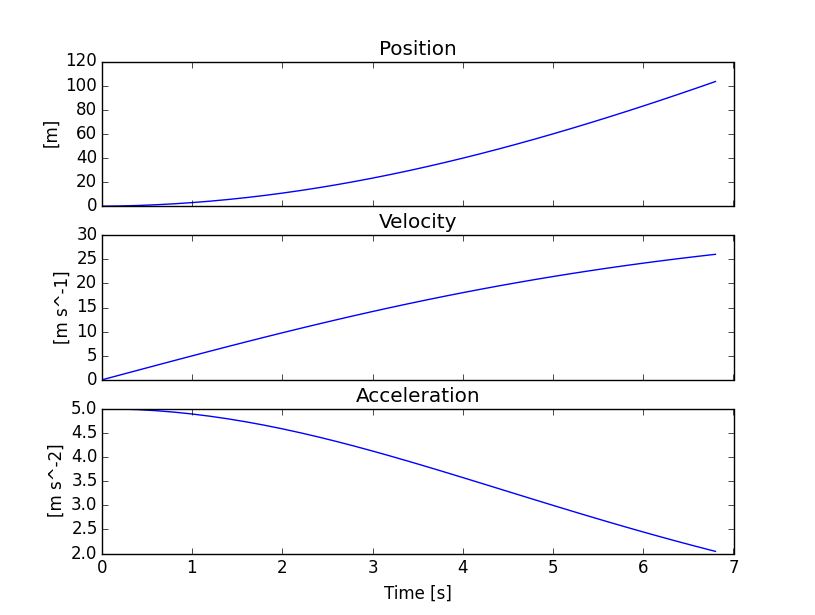
\includegraphics[scale=0.8]{e.png} 
        \caption{Graphs showing the position, velocity and acceleration of the sprinter.}
        \label{fig:e}
\end{figure}

\begin{figure}[H]
        \centering 
        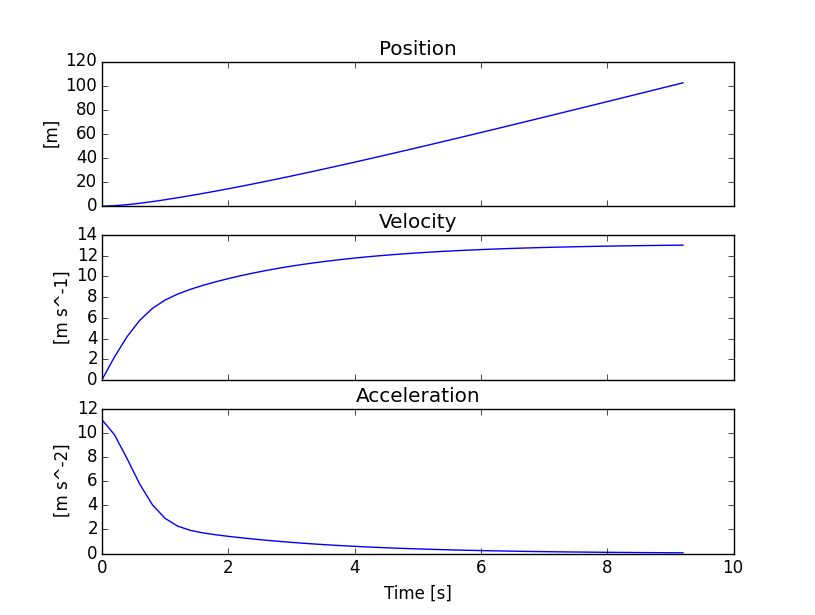
\includegraphics[scale=0.8]{i.png} 
        \caption{Graphs showing the position, velocity and acceleration of the sprinter with the modified method}
        \label{fig:i}
\end{figure}

\begin{figure}[H]
        \centering 
        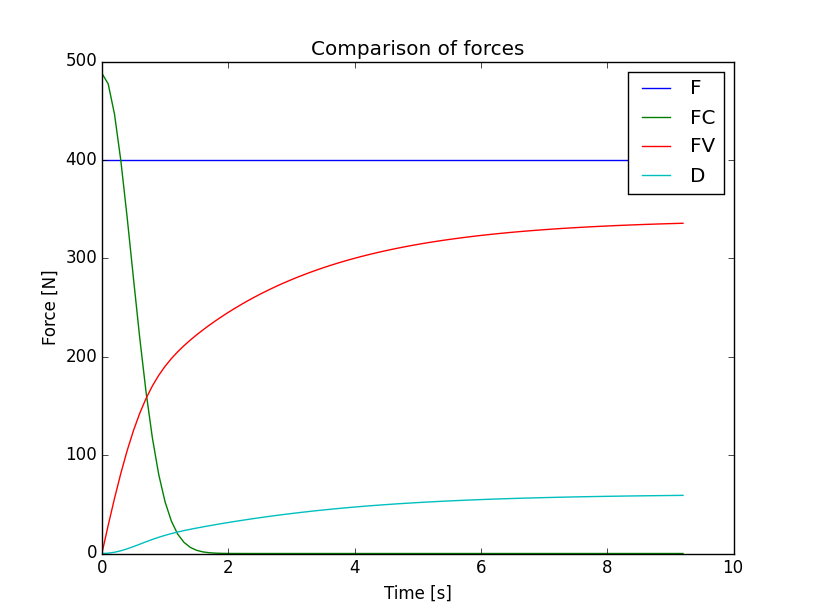
\includegraphics[scale=0.8]{k.png} 
        \caption{Comparison of the forces acting on the runner}
        \label{fig:k}
\end{figure}


\section{Source code}
\lstinputlisting{e.py}

\end{document}
